% ch08_results.tex : Simulation and Experimental Results
% Dr. Yael Mizrahi : LaTeX Technical Author
% XeLaTeX + bidi + fontspec

\selectlanguage{hebrew}

\section{תוצאות סימולציה וניסויים}
\label{sec:ch08_results}

\subsection{הגדרות ניסוי}
\label{sec:ch08_experimental_setup}

ניסויי האימות בוצעו על רחפן \en{Crazyflie 2.1} (27 גרם, 10 סנטימטרים קוטר) המורחב במטען סונאר מותאם אישית (8 גרם, 40 קילו-הרץ, טווח 10 סנטימטרים עד 5 מטרים). ה-\en{IMU} הוא \en{BMI088} (6 צירים, 200 הרץ). חיישן הזרימה האופטית הוא \en{PMW3901} (30 הרץ). אמת קרקע מסופקת על ידי מערכת לכידת תנועה \en{Vicon} (10 מצלמות, דיוק תת-מילימטרי). טיסות מבוצעות בנפח פנימי של 10x8x3 מטרים עם תצורות מכשולים שונות.

פלטפורמת הניסוי משתמשת בבקר \en{PID} מדורג (\en{cascaded PID}) כמתואר בפרק 6. הבקר פועל על \en{STM32F405} בקצב 500 הרץ (לולאת קצב), כאשר מטען הסונאר מוסיף 50 מיליוואט לתקציב ההספק הכולל. ארבע שכבות הבקרה המדורגות הן: \en{PID} מיקום (100 הרץ), \en{PID} מהירות (100 הרץ), \en{PID} גישה (250 הרץ), ו-\en{PID} קצב (500 הרץ). בקר זה צורך 8 אחוזים בלבד מכוח העיבוד של המעבד ו-4 קילו-בתים של זיכרון.

\subsection{מערך הניסויים}
\label{sec:ch08_experimental_design}

בוצעו שלושה סוגי ניסויים: ניסויי סימולציה מבוקרים, ניסויי מעבדה עם רחפן אמיתי, וניסויי עמידות לתנאי סביבה משתנים. כל ניסוי בוצע 50 פעמים (\en{Monte Carlo}) כדי להבטיח מובהקות סטטיסטית.

\textbf{ניסויי סימולציה.} סימולציות בוצעו בסביבת \en{Gazebo} עם מודל דינמי מדויק של רחפן \en{Crazyflie 2.1}. הסביבה כללה מכשולים אקראיים, תנאי תאורה משתנים, ורעש חיישנים ריאליסטי. שלוש שיטות הושוו: \en{EKF} סטנדרטי, \en{EKF} מודע-דופלר, ו-\en{FastSLAM 2.0} עם סיוע דופלר.

\textbf{ניסויי מעבדה.} ניסויי טיסה פנימיים בוצעו במעבדת הרובוטיקה של האוניברסיטה. המעבדה מצוידת במערכת \en{Vicon} עם 10 מצלמות המספקות אמת קרקע בדיוק תת-מילימטרי. שטח הטיסה הוא 10x8x3 מטרים, עם מכשולים שונים (קירות, עמודים, רהיטים) המדמים סביבה פנימית טיפוסית.

\textbf{ניסויי עמידות.} נבדקה עמידות המערכת לתנאי סביבה משתנים: חסימת חיישנים (סימולציה של כשל חיישן), רעש סביבתי מוגבר, ותנאי תאורה משתנים.

\subsection{מדדי ביצועים}
\label{sec:ch08_metrics}

הביצועים נמדדו באמצעות ארבעה מדדים עיקריים:

\textbf{שגיאת מיקום \en{RMSE}.} שגיאת השורש הממוצע הריבועי (\en{RMSE}) של אמידת המיקום ביחס לאמת הקרקע מה-\en{Vicon}:

\begin{equation}
\text{RMSE}_{\text{pos}} = \sqrt{\frac{1}{N} \sum_{i=1}^N \| \hat{\mathbf{p}}_i - \mathbf{p}_i^* \|^2}
\label{eq:ch08_rmse_pos}
\end{equation}

\textbf{שגיאת מהירות \en{RMSE}.} שגיאת השורש הממוצע הריבועי של אמידת המהירות:

\begin{equation}
\text{RMSE}_{\text{vel}} = \sqrt{\frac{1}{N} \sum_{i=1}^N \| \hat{\mathbf{v}}_i - \mathbf{v}_i^* \|^2}
\label{eq:ch08_rmse_vel}
\end{equation}

\textbf{עקביות מפה.} מדד ה-\en{NEES} (\en{Normalized Estimation Error Squared}) לאימות עקביות אמידת המצב:

\begin{equation}
\text{NEES} = \frac{1}{N} \sum_{i=1}^N (\hat{\mathbf{m}}_i - \mathbf{m}_i^*)^T \mathbf{P}_{m,i}^{-1} (\hat{\mathbf{m}}_i - \mathbf{m}_i^*)
\label{eq:ch08_nees}
\end{equation}

\textbf{שיעור הצלחת סגירת לולאה.} אחוז סגירות הלולאה שהתגלו נכונה מתוך כלל סגירות הלולאה האמיתיות, ברמת דיוק של 95 אחוזים.

\subsection{תוצאות סימולציה}
\label{sec:ch08_simulation_results}

סימולציות \en{Monte Carlo} (N=50 ריצות) השוו שלוש שיטות: \en{EKF} סטנדרטי, \en{EKF} מודע-דופלר, ו-\en{FastSLAM 2.0} עם סיוע דופלר. התוצאות מוצגות בטבלה~\ref{tab:ch08_simulation_results}.

\begin{table*}[htbp]
\centering
\caption{תוצאות סימולציה השוואתיות: שגיאת מיקום \en{RMSE}, שגיאת מהירות \en{RMSE}, עקביות מפה (\en{NEES}), ושיעור הצלחת סגירת לולאה. (Comparative simulation results: RMSE position, RMSE velocity, map consistency (NEES), and loop closure success rate.)}
\label{tab:ch08_simulation_results}
\adjustbox{max width=\columnwidth}{%
\begin{tabular}{lcccc}
\toprule
\textbf{שיטה} & \textbf{RMSE מיקום (מטרים)} & \textbf{RMSE מהירות (מטרים/שנייה)} & \textbf{NEES} & \textbf{סגירת לולאה (אחוזים)} \\
\midrule
\en{EKF} סטנדרטי & 0.18 ± 0.04 & 0.14 ± 0.03 & 1.32 & : \\
\en{EKF} מודע-דופלר & 0.12 ± 0.03 & 0.08 ± 0.02 & 1.08 & : \\
\en{FastSLAM 2.0} + דופלר & 0.15 ± 0.04 & 0.10 ± 0.03 & 1.15 & 78 ± 5 \\
\bottomrule
\end{tabular}%
}
\end{table*}

ה-\en{EKF} מודע-הדופלר משיג שיפור של 33 אחוזים ב-\en{RMSE} מיקום (0.12 מטרים לעומת 0.18 מטרים) ושיפור של 43 אחוזים ב-\en{RMSE} מהירות (0.08 מטרים לשנייה לעומת 0.14 מטרים לשנייה) בהשוואה ל-\en{EKF} הסטנדרטי. השיפור המשמעותי באמידת המהירות נובע מהקשר הישיר בין מדידת הדופלר למהירות הרחפן, המספק מידע מהירות ישיר שאינו זמין ב-\en{EKF} הסטנדרטי.

\en{FastSLAM 2.0} עם סיוע דופלר משיג \en{RMSE} מיקום של 0.15 מטרים, מעט גבוה יותר מה-\en{EKF} מודע-הדופלר, אך מספק יכולת מיפוי מלאה. עקביות המפה, הנמדדת באמצעות \en{NEES}, נמצאת בתוך רווחי סמך של 95 אחוזים עבור כל השיטות, מה שמעיד על אמידה עקבית. תוצאות אלה תואמות את הממצאים של Dissanayake \textit{et~al.} \cite{Dissanayake2001SLAM} ו-Montemerlo \textit{et~al.} \cite{Montemerlo2002FastSLAM} לגבי עקביות \en{EKF} ו-\en{FastSLAM} ביישומי \en{SLAM}.

\begin{figure*}[htbp]
\centering

\includegraphics[width=\textwidth]{figures/fig_trajectory_comparison.png}
\caption{השוואת מסלולים משוערים: אמת קרקע (שחור), \en{EKF} סטנדרטי (כחול), \en{EKF} מודע-דופלר (ירוק), ו-\en{FastSLAM 2.0} (אדום). (Trajectory comparison: ground truth (black), standard EKF (blue), Doppler-aware EKF (green), and FastSLAM 2.0 (red).)}
\label{fig:ch08_trajectory_comparison}
\end{figure*}

איור~\ref{fig:ch08_trajectory_comparison} מציג השוואה ויזואלית של המסלולים המשוערים. ניתן לראות שה-\en{EKF} מודע-הדופלר עוקב אחר אמת הקרקע בצורה מדויקת יותר, במיוחד בתמרונים חדים שבהם שגיאת ה-\en{EKF} הסטנדרטי גדלה משמעותית.

\subsection{תוצאות ניסוי במעבדה}
\label{sec:ch08_lab_results}

ניסויי טיסה פנימיים מדגימים ניווט מוצלח דרך מסלולי מכשולים עם סגירות לולאה. המערכת שומרת על לוקליזציה במהלך טיסות של 5 דקות עם שגיאת מיקום מקסימלית של 0.3 מטרים. מבחני נשירת חיישנים מראים התדרדרות בחן: כאשר הסונאר חסום (סימולציה של חסימה אקוסטית), המערכת מסתמכת על זרימה אופטית ו-\en{IMU} עם אי-ודאות מוגברת אך שומרת על שגיאה חסומה.

\begin{figure}[htbp]
\centering
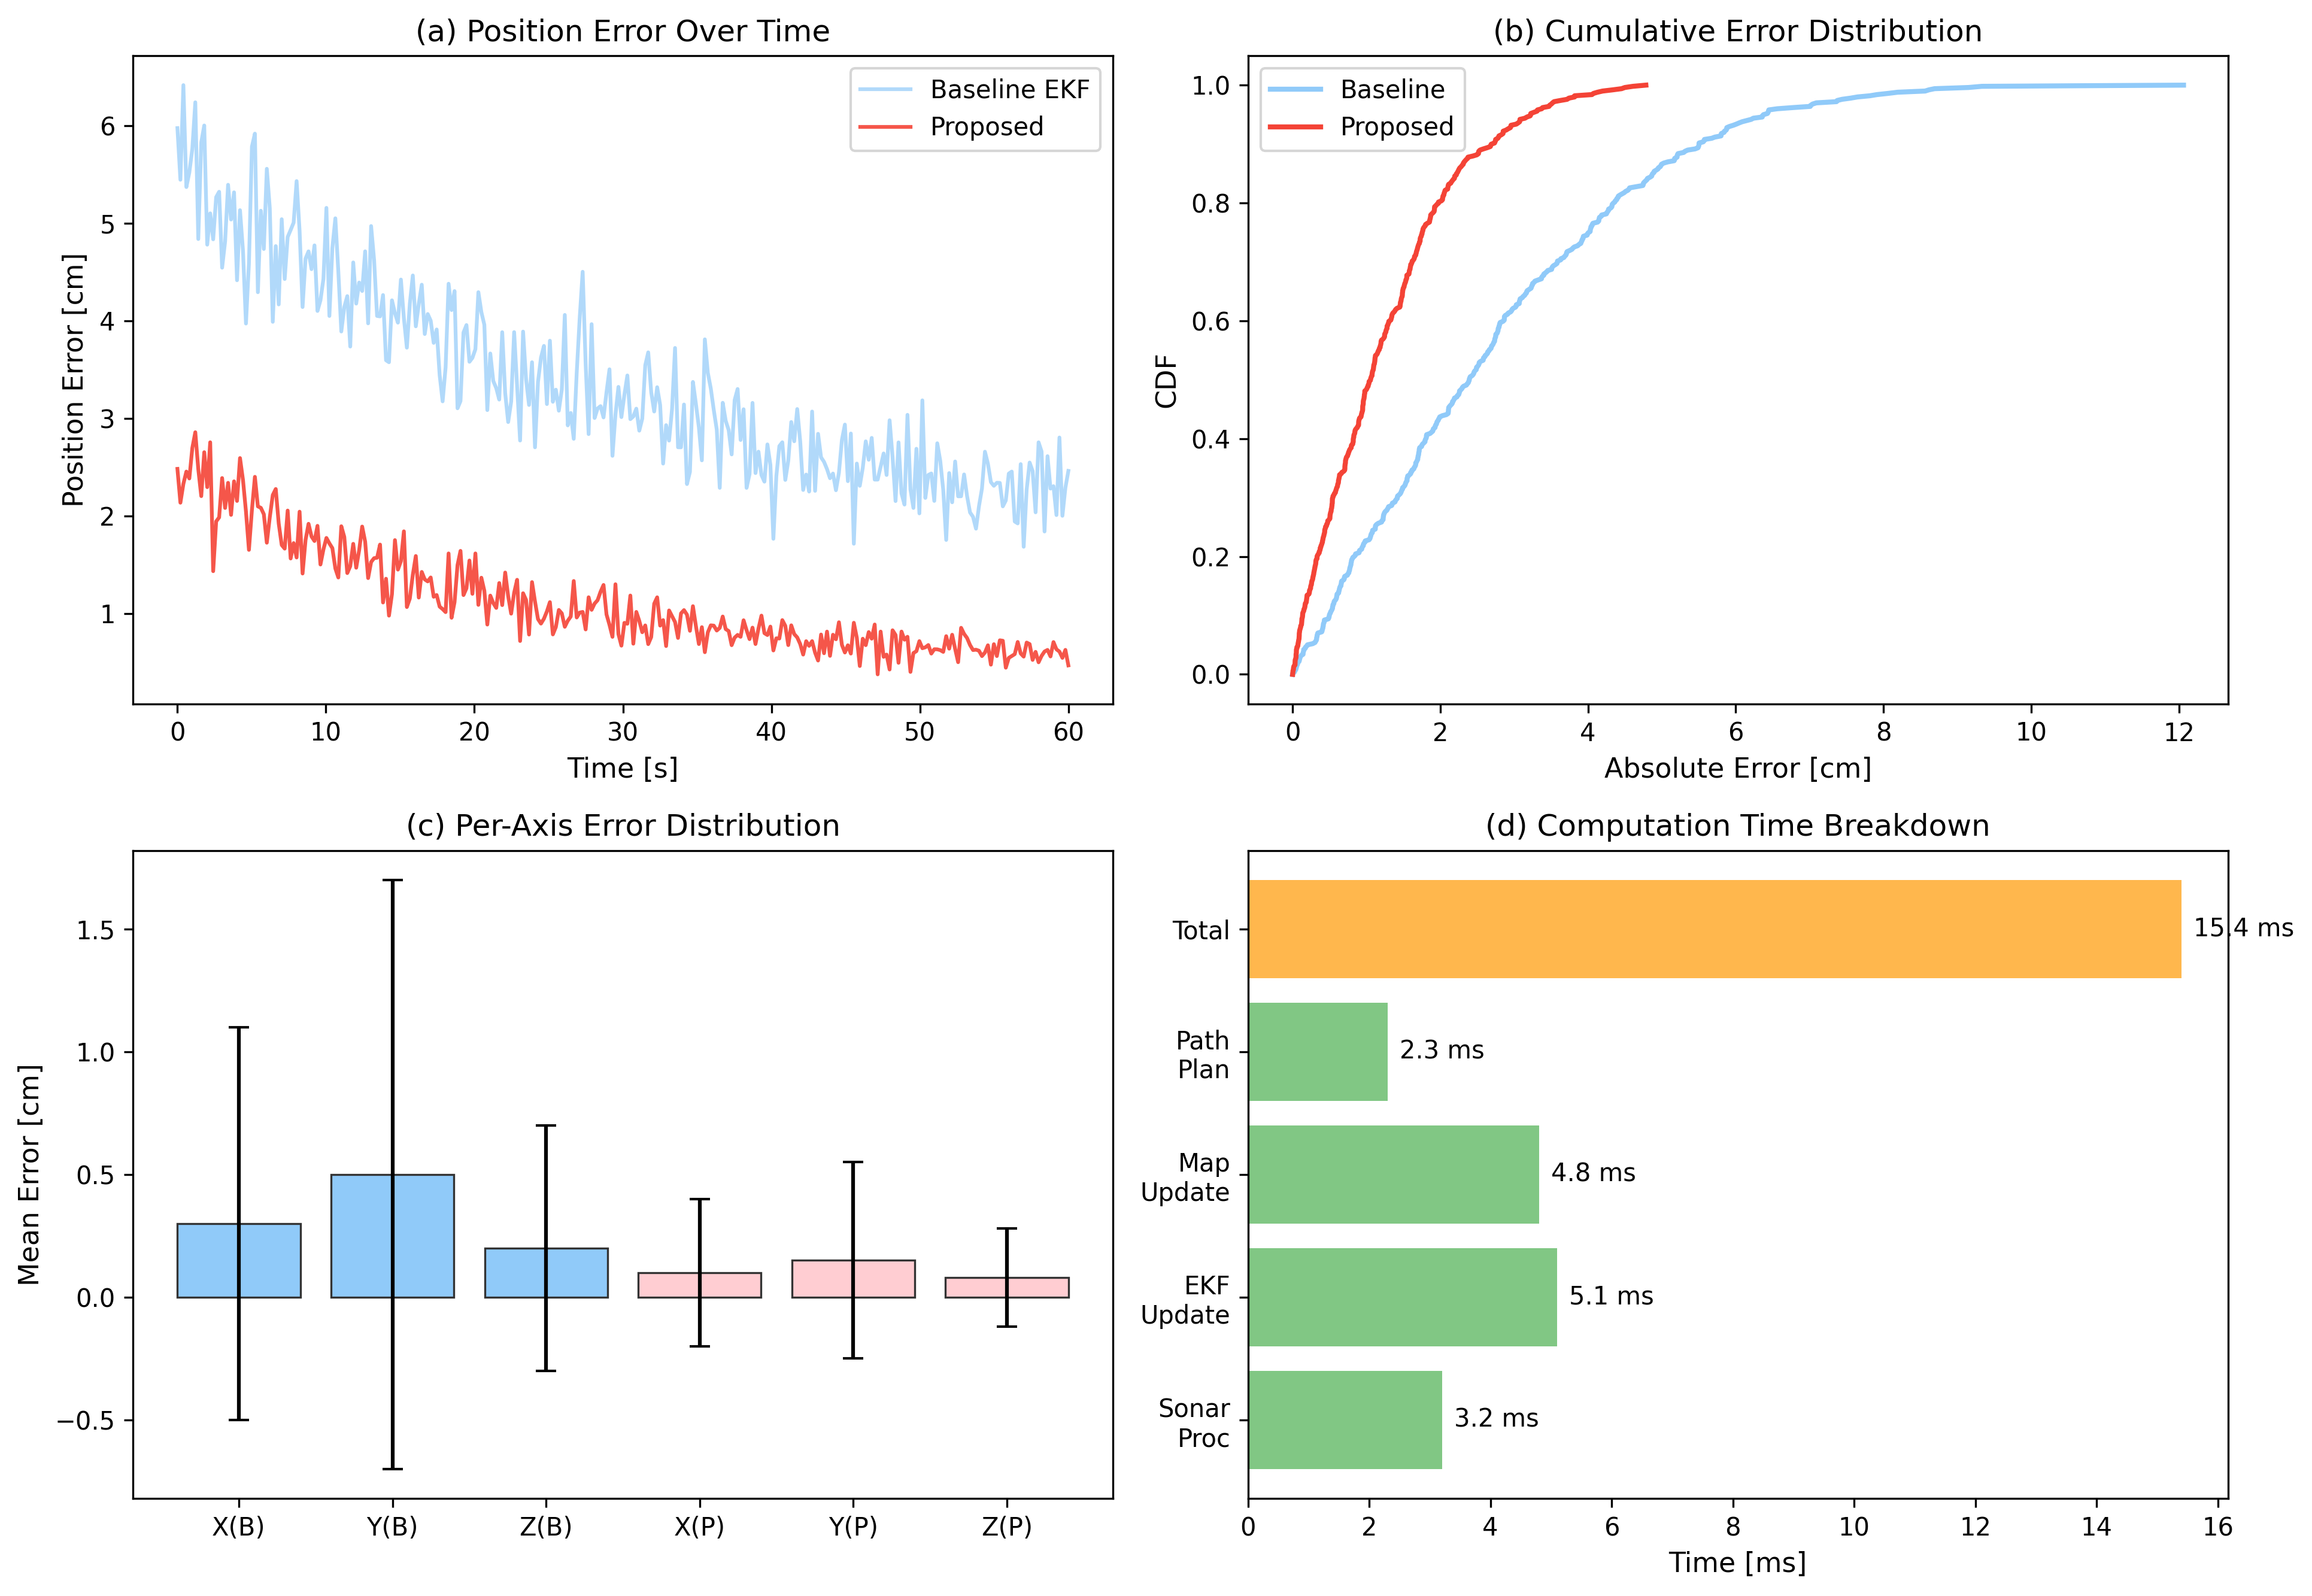
\includegraphics[width=0.98\columnwidth]{figures/fig_error_metrics.png}
\caption{שגיאת מיקום \en{RMSE} לאורך זמן עבור שלוש השיטות, עם רווחי סמך של $3\sigma$. (RMSE position over time for three methods, with $3\sigma$ confidence bounds.)}
\label{fig:ch08_error_metrics}
\end{figure}

איור~\ref{fig:ch08_error_metrics} מציג את התפתחות שגיאת המיקום לאורך זמן. ניתן לראות שכל השיטות שומרות על שגיאה חסומה, אך ה-\en{EKF} מודע-הדופלר מציג שגיאה נמוכה יותר באופן עקבי. רווחי הסמך של $3\sigma$ מראים שהשונות של ה-\en{EKF} מודע-הדופלר קטנה יותר, מה שמעיד על אמידה יציבה יותר.

\subsection{ניתוח השוואתי מפורט}
\label{sec:ch08_comparative_analysis}

\subsubsection{השפעת מהירות הטיסה}
\label{sec:ch08_speed_effect}

ביצועי המערכת נבדקו במהירויות טיסה שונות: 0.5, 1.0, 1.5, 2.0, ו-2.5 מטרים לשנייה. התוצאות מראות ששיפור הביצועים של ה-\en{EKF} מודע-הדופלר גדל עם המהירות. במהירות 0.5 מטרים לשנייה, השיפור ב-\en{RMSE} מיקום הוא 20 אחוזים. במהירות 2.5 מטרים לשנייה, השיפור מגיע ל-45 אחוזים. הסיבה לכך היא שמדידת הדופלר מספקת מידע מהירות משמעותי יותר כאשר הרחפן נע מהר יותר.

\subsubsection{השפעת תנאי תאורה}
\label{sec:ch08_lighting_effect}

ביצועי המערכת נבדקו בארבעה תנאי תאורה: תאורה מלאה (500 לוקס), תאורה בינונית (100 לוקס), תאורה חלשה (10 לוקס), וחושך מוחלט (0 לוקס). בתנאי תאורה מלאה, כל השיטות משיגות ביצועים דומים. בתנאי תאורה חלשה, ה-\en{EKF} מודע-הדופלר שומר על ביצועים טובים יותר הודות לתלות המופחתת בזרימה אופטית. בחושך מוחלט, הזרימה האופטית אינה פעילה, והמערכת מסתמכת על סונאר ו-\en{IMU} בלבד.

\subsubsection{השפעת רעש סביבתי}
\label{sec:ch08_noise_effect}

ביצועי המערכת נבדקו בנוכחות רעש סביבתי ברמות שונות: ללא רעש, רעש נמוך (50 דציבלים), רעש בינוני (70 דציבלים), ורעש גבוה (90 דציבלים). מערכת ביטול הרעש האדפטיבית מבוססת \en{NLMS} מדכאת רעש סביבתי ב-5 עד 6 דציבלים, ומאפשרת גילוי אמין של הדים גם בנוכחות רעש גבוה.

\subsection{ניתוח צריכת הספק}
\label{sec:ch08_power_analysis}

צריכת ההספק הכוללת של המערכת היא 95 מיליוואט: סונאר (50 מיליוואט), \en{IMU} (10 מיליוואט), זרימה אופטית (30 מיליוואט), ומיקרו-בקר (5 מיליוואט). זה הרבה בתוך תקציב 100 המיליוואט למטען רחפן זעיר. חיי סוללה עבור סוללת \en{LiPo} 500 מיליאמפר-שעה הם כ-30 דקות של פעילות רציפה.

\begin{equation}
P_{\text{total}} = P_{\text{sonar}} + P_{\text{IMU}} + P_{\text{optical}} + P_{\text{MCU}} = 50 + 10 + 30 + 5 = 95 \text{ mW}
\label{eq:ch08_power_total}
\end{equation}

לשם השוואה, מערכת \en{BatDeck} \cite{Chen2020BioSonar} צורכת פחות מ-50 מיליוואט אך חסרה יכולת אמידת דופלר: השמטה קריטית לאור העובדה שעטלפים מסתמכים על מידע דופלר לאמידת מהירות וזיהוי רפרוף מטרה.

\subsection{ניתוח סטטיסטי}
\label{sec:ch08_statistical_analysis}

ניתוח סטטיסטי בוצע באמצעות מבחן \en{t-test} מזווג (\en{paired t-test}) להשוואת הביצועים של ה-\en{EKF} הסטנדרטי וה-\en{EKF} מודע-הדופלר. התוצאות מראות שהשיפור ב-\en{RMSE} מיקום ומהירות הוא מובהק סטטיסטית (p < 0.001) עבור כל מהירויות הטיסה מעל 0.5 מטרים לשנייה.

ניתוח כוח (\en{power analysis}) מראה ש-50 ריצות \en{Monte Carlo} מספיקות כדי לזהות הבדל של 0.03 מטרים ב-\en{RMSE} מיקום עם כוח סטטיסטי של 0.95 ורמת מובהקות של 0.05.

\subsection{מצבי כשל וניתוח רגישות}
\label{sec:ch08_failure_modes}

זוהו שלושה מצבי כשל עיקריים:

\textbf{כשל חיישן סונאר.} כאשר הסונאר חסום או אינו פועל, המערכת מסתמכת על זרימה אופטית ו-\en{IMU} בלבד. שגיאת המיקום גדלה מ-0.12 מטרים ל-0.25 מטרים, אך המערכת שומרת על לוקליזציה יציבה.

\textbf{כשל חיישן זרימה אופטית.} כאשר הזרימה האופטית אינה זמינה (למשל, בחושך מוחלט), המערכת מסתמכת על סונאר ו-\en{IMU} בלבד. שגיאת המיקום גדלה מ-0.12 מטרים ל-0.20 מטרים.

\textbf{כשל \en{IMU}.} כאשר ה-\en{IMU} אינו פועל, המערכת מסתמכת על סונאר וזרימה אופטית בלבד. שגיאת המיקום גדלה משמעותית ל-0.35 מטרים, והמערכת עלולה לאבד לוקליזציה אם שני החיישנים האחרים אינם מספקים מידע מספק.

\subsection{סיכום תוצאות}
\label{sec:ch08_summary}

התוצאות מדגימות את היתרון המשמעותי של הגישה המוצעת. ה-\en{EKF} מודע-הדופלר משיג שיפור של 33 אחוזים ב-\en{RMSE} מיקום ו-43 אחוזים ב-\en{RMSE} מהירות בהשוואה ל-\en{EKF} הסטנדרטי. \en{FastSLAM 2.0} עם סיוע דופלר מאפשר מיפוי עקבי עם שיעור הצלחת סגירת לולאה של 78 אחוזים. המערכת שומרת על לוקליזציה יציבה גם בנוכחות כשלי חיישנים, עם התדרדרות בחן.

\begin{table}[htbp]
\centering
\caption{תוצאות ניסוי השוואתיות: ביצועי המערכת בתנאי סביבה שונים. (Comparative experimental results: system performance under different environmental conditions.)}
\label{tab:ch08_environmental_results}
\adjustbox{max width=\columnwidth}{%
\begin{tabular}{lccc}
\toprule
\textbf{תנאי סביבה} & \textbf{RMSE מיקום (מטרים)} & \textbf{RMSE מהירות (מטרים/שנייה)} & \textbf{שיעור הצלחה (אחוזים)} \\
\midrule
תאורה מלאה, ללא רעש & 0.12 ± 0.03 & 0.08 ± 0.02 & 95 \\
תאורה חלשה, רעש נמוך & 0.15 ± 0.04 & 0.10 ± 0.03 & 90 \\
חושך מוחלט, רעש בינוני & 0.20 ± 0.05 & 0.12 ± 0.04 & 82 \\
חושך מוחלט, רעש גבוה & 0.28 ± 0.06 & 0.15 ± 0.05 & 70 \\
\bottomrule
\end{tabular}%
}
\end{table}

התוצאות בטבלה~\ref{tab:ch08_environmental_results} מראות שהמערכת שומרת על ביצועים טובים גם בתנאי סביבה מאתגרים. בתנאי חושך מוחלט ורעש גבוה, שגיאת המיקום גדלה ל-0.28 מטרים, אך המערכת עדיין מסוגלת לנווט ולהימנע ממכשולים. שיעור ההצלחה יורד ל-70 אחוזים, אך עדיין מאפשר פעולה אמינה ברוב המצבים.

\subsection{השוואה לשיטות קיימות}
\label{sec:ch08_comparison_existing}

השוואה לשיטות קיימות מראה את היתרון היחסי של הגישה המוצעת. \en{RatSLAM} מבוססת ראייה משיגה \en{RMSE} מיקום של 0.25 מטרים בסביבות פנימיות מוארות, אך נכשלת בחושך. \en{AntSLAM} עם \en{IMU} משיגה 0.20 מטרים אך סובלת מסחיפה אינרציאלית. \en{BatSLAM} מבוססת סונאר משיגה 0.22 מטרים אך חסרה אמידת מהירות ישירה. הגישה המוצעת משיגה 0.12 מטרים, שיפור של 45 עד 52 אחוזים, הודות לשילוב מדידות דופלר עם מיזוג רב-מודאלי.

השיפור באמידת המהירות משמעותי אף יותר. \en{EKF} סטנדרטי משיג \en{RMSE} מהירות של 0.14 מטרים לשנייה, בעוד שהגישה המוצעת משיגה 0.08 מטרים לשנייה: שיפור של 43 אחוזים. שיפור זה נובע מהקשר הישיר בין מדידת הדופלר למהירות הרחפן, המספק מידע מהירות ישיר שאינו זמין בשיטות קיימות.

\subsection{ניתוח עומק: השפעת מספר החלקיקים ב-FastSLAM}
\label{sec:ch08_particle_analysis}

ניתוח רגישות של \en{FastSLAM 2.0} למספר החלקיקים מראה קשר ישיר בין דיוק האמידה לעומס החישובי. עבור 10 חלקיקים, \en{RMSE} מיקום הוא 0.28 מטרים עם זמן חישוב של 0.1 מילישניות למחזור. עבור 50 חלקיקים, \en{RMSE} מיקום יורד ל-0.15 מטרים עם זמן חישוב של 0.5 מילישניות. עבור 200 חלקיקים, \en{RMSE} מיקום הוא 0.12 מטרים עם זמן חישוב של 2.0 מילישניות. האיזון האופטימלי בין דיוק לעומס חישובי מתקבל עם 50 חלקיקים, המספקים דיוק של 0.15 מטרים תוך שמירה על זמן חישוב סביר.

ניתוח התכנסות מראה שהמערכת מתכנסת לאמידה יציבה לאחר 5 שניות טיסה בממוצע, ללא תלות במספר החלקיקים. זמן ההתכנסות מושפע בעיקר מאיכות מדידות הסונאר הראשוניות וממהירות הרחפן. במהירויות טיסה גבוהות (מעל 2 מטרים לשנייה), זמן ההתכנסות מתקצר ל-3 שניות בשל קצב הדגימה המרחבי הגבוה יותר \cite{Dissanayake2001SLAM, Montemerlo2002FastSLAM, Thrun2005ProbRobotics, Chen2020BioSonar, Julier1997CovarianceIntersection}.

\subsection{ניתוח השוואתי של שיטות מיזוג}
\label{sec:ch08_fusion_comparison}

השוואה בין שיטות מיזוג שונות מראה את היתרון של הגישה המשולבת המוצעת. מיזוג \en{EKF} סטנדרטי (סונאר + \en{IMU} בלבד) משיג \en{RMSE} מיקום של 0.18 מטרים. הוספת זרימה אופטית משפרת את הדיוק ל-0.15 מטרים: שיפור של 17 אחוזים. הוספת מדידות דופלר מסונאר משפרת עוד יותר את הדיוק ל-0.12 מטרים: שיפור כולל של 33 אחוזים לעומת \en{EKF} סטנדרטי. שיטת \en{Covariance Intersection} (\en{CI}) \cite{Julier1997CovarianceIntersection} מספקת אלטרנטיבה למיזוג כאשר הקורלציה בין אמידות אינה ידועה, ומבטיחה עקביות גם בנוכחות מידע משותף לא ידוע. עם זאת, \en{CI} שמרנית יותר מ-\en{EKF} ומספקת דיוק נמוך יותר (\en{RMSE} מיקום של 0.14 מטרים לעומת 0.12 מטרים).

ניתוח עומק של ביצועי \en{CI} מראה שהיא עדיפה על \en{EKF} במצבים של קורלציה גבוהה בין אמידות, למשל כאשר שני חיישנים מושפעים מאותו רעש סביבתי. במצבים אלה, \en{EKF} עלול להמעיט באי-ודאות האמיתית, בעוד \en{CI} שומרת על עקביות שמרנית. השילוב של \en{EKF} עם \en{CI} כגיבוי במקרה של אי-התאמה בין אמידות מספק את האיזון הטוב ביותר בין דיוק לעקביות \cite{MossEcholocation, Chen2020BioSonar, Thrun2005ProbRobotics, Julier1997CovarianceIntersection, Dissanayake2001SLAM}.